\documentclass[12pt]{article}

\include{preamble}
\usepackage{pgfplots}
\pgfmathdeclarefunction{gauss}{2}
{\pgfmathparse{1/(#2*sqrt(2*pi))*exp(-((x-#1)^2)/(2*#2^2))}}


\newtoggle{professormode}
%\toggletrue{professormode} %STUDENTS: DELETE or COMMENT this line



\title{MATH 390.4 / 650.2 Spring 2018 Homework \#3t}

\author{Darshan Patel} %STUDENTS: write your name here

\iftoggle{professormode}{
\date{Due 11:59PM Friday, March 23, 2018 under the door of KY604 \\ \vspace{0.5cm} \small (this document last updated \today ~at \currenttime)}
}

\renewcommand{\abstractname}{Instructions and Philosophy}

\begin{document}
\maketitle

\iftoggle{professormode}{
\begin{abstract}
The path to success in this class is to do many problems. Unlike other courses, exclusively doing reading(s) will not help. Coming to lecture is akin to watching workout videos; thinking about and solving problems on your own is the actual ``working out.''  Feel free to \qu{work out} with others; \textbf{I want you to work on this in groups.}

Reading is still \textit{required}. For this homework set, read about all the concepts introduced in class online e.g. multivariate least squares linear modeling, orthogonal projections, QR decomposition, etc. This is your responsibility to supplement in-class with your own readings. Also, read ch 2 in Silver and 2--4 in Finlay.

The problems below are color coded: \ingreen{green} problems are considered \textit{easy} and marked \qu{[easy]}; \inorange{yellow} problems are considered \textit{intermediate} and marked \qu{[harder]}, \inred{red} problems are considered \textit{difficult} and marked \qu{[difficult]} and \inpurple{purple} problems are extra credit. The \textit{easy} problems are intended to be ``giveaways'' if you went to class. Do as much as you can of the others; I expect you to at least attempt the \textit{difficult} problems. 

This homework is worth 100 points but the point distribution will not be determined until after the due date. See syllabus for the policy on late homework.

Up to 10 points are given as a bonus if the homework is typed using \LaTeX. Links to installing \LaTeX~and program for compiling \LaTeX~is found on the syllabus. You are encouraged to use \url{overleaf.com}. If you are handing in homework this way, read the comments in the code; there are two lines to comment out and you should replace my name with yours and write your section. The easiest way to use overleaf is to copy the raw text from hwxx.tex \emph{and} preamble.tex into two new overleaf tex files with the same name. If you are asked to make drawings, you can take a picture of your handwritten drawing and insert them as figures or leave space using the \qu{$\backslash$vspace} command and draw them in after printing or attach them stapled.

The document is available with spaces for you to write your answers. If not using \LaTeX, print this document and write in your answers. I do not accept homeworks which are \textit{not} on this printout. Keep this first page printed for your records.

\end{abstract}

\thispagestyle{empty}
\vspace{1cm}
NAME: \line(1,0){380}
\clearpage
}

\problem{These are questions about Silver's book, chapter 2.}


\begin{enumerate}

\intermediatesubproblem{If one's goal is to fit a model for a phenomenon $y$, what is the difference between the approaches of the hedgehog and the fox? Answer using notation from class (i.e. $t ,f, g, h^*, \delta, \epsilon, e, t, z_1, \ldots, z_t, \mathbb{D}, \mathcal{H}, \mathcal{A}, \mathcal{X}, \mathcal{Y}, X, y, n, p, x_{\cdot 1}, \ldots, x_{\cdot p}, x_{1 \cdot}, \ldots, x_{n \cdot}$, etc.). Connecting this to the modeling framework should really make you think about what Tetlock's observation means for political and historical phenomena.}\spc{4} \\
The difference between the approaches of the hedgehog and the fox is that the fox demonstrated the ability to make predictions using a multitude of approaches toward a problem, whereas the hedgehog only does no better than random chance. In notation form, the hedgehog's approach is $\bar{x}$ while the fox's approach is $\mathcal{A}(\mathcal{D},\mathcal{H})$. 


\easysubproblem{Why did Harry Truman like hedgehogs? Are there a lot of people that think this way?}\spc{4} \\
Harry Truman liked hedgehogs because they gave simple one answers whereas foxes couldn't give a concise answer. A lot of people don't think like hedgehogs because they usually create predictions from data and not from a random guess. 


\hardsubproblem{Why is it that the more education one acquires, the less accurate one's predictions become?}\spc{4} \\ 
The more education that one acquires, the less accurate its' predictions become due to the accumulation of bias. With the information it receives, it can change them to confirm its bias. It can add more noise to all the information at hand and can disturb the ability to make an accurate prediction. 

\easysubproblem{Why are probabilistic classifiers (i.e. algorithms that output functions that return probabilities) better than vanilla classifiers (i.e. algorithms that only return the class label)? We will move in this direction in class soon.}\spc{4} \\
Probabilistic classifiers are better than vanilla classifiers because they don't return a clear image of the predictions but rather the chance of something occurring. Rather than saying which value is predicted, it allows for probability to dictate the chance of different outcomes occurring. 

\end{enumerate}

\problem{These are questions about Finlay's book, chapter 2-4. We will hold off on chapter 1 until we cover probability estimation after midterm 2.}


\begin{enumerate}

\easysubproblem{What term did we use in class for \qu{behavioral (outcome) data}?}\spc{0}
\\ phenomenon.

\easysubproblem{Write about some reasons why data scientists implement models that are subpar in predictive performance (p27).}\spc{3} \\
Models that are subpar in predictive performance will be implemented sometimes to respect business requirements and constraints. It is also common for models to be simple for the regular laymen to understand and implement. 

\easysubproblem{In the first wine example, what is the outcome metric and what kind of supervised learning was employed?}\spc{0} \\
The outcome metric is a classification model, a table of values showcasing responses and the score distribution amongst people who had different scores.  It was employed using a decision tree algorithm. 

\easysubproblem{In the second wine example, what is the outcome metric and kind of supervised learning was employed?}\spc{0} \\
The outcome metric is a regression model, a table that predicts the gross profit collected given the score. It was also employed using a decision tree algorithm.

\easysubproblem{In the third chapter, why is it that some organizations cannot use predictive modeling to improve their business?}\spc{3} \\
Some businesses cannot use predictive modeling to improve their business because it is not accepted by the entire organization. Not everyone from the senior manager to front line staff is comfortable acting upon the decisions made by the predictive model. 

\easysubproblem{In the bankruptcy case, what is the problem with merely using $g$ to obtain a $\hat{y}$ without any other information from the model?}\spc{3} \\
By not using other information from the model, a proper assessment of the model and outcome cannot be created. People will use their own judgement if they are confused about what's in the model and whether it is useful or not.

\easysubproblem{Chapter 3 talks about using the model with human judgment. Under what circumstances is this beneficial? Answer using notation from class (i.e. $t ,f, g, h^*, \delta, \epsilon, e, t$, $z_1, \ldots, z_t, \mathbb{D}, \mathcal{H}, \mathcal{A}, \mathcal{X}, \mathcal{Y}, X, y, n, p, x_{\cdot 1}, \ldots, x_{\cdot p}, x_{1 \cdot}, \ldots, x_{n \cdot}$, etc.).}\spc{3} \\
It is beneficial to use models with human judgment when you have experience or biases. This is referred to as $e$, the difference between the true result you believe in which differs from the result made by the model.

\hardsubproblem{In Chapter 4 Finaly makes an interesting observation based on his experience in data science. He says most predictive models have $p \leq 30$. Why do you think this is? Discuss.}\spc{5} \\
Most predictive models have $p \leq 30$. This is a good constraint to have. If you have too many variables to measure a phenomenon, you can run into different situations where one variable will have an impact on another and are thus not independent. Perhaps you will see that there is no clear conclusion that can be made from more than $30$ factors about a phenomenon. Each variable may not be independent of another or play little role if any. 


\easysubproblem{He says there is \qu{almost always other data that could be acquired ... [which] doesn't always come for free}. The \qu{data} he is talking about here specifically means \qu{more predictors} i.e. increasing $p$. In what cases would someone be willing to pay for this data?}\spc{3} \\
Someone would be willing to pay for \qu{more predictors} if it can be proved that the predictors can create a clear model of the phenomenon. If the value of the data can be determined to be a lot, then it will be purchased. A situation of this is when a social media network sells your data to an advertising company to determine when to show which ads to users to bring in the most profit, \qu{clicks}, to the advertising company. 

\easysubproblem{Table 4 lists \qu{data types} about what type of observations?}\spc{1} \\
categorical observations.

\easysubproblem{What type of data does he find in his experience to be the most important to predictive modeling? Why do you think this is so?}\spc{3} \\
The most important type of data in predictive modeling, according to Finaly, is data about primary behavior. This should be the most important because your behavior can dictate your future behaviors. It is common to predict something that you already do. 

\easysubproblem{If $x_{\cdot 17}$ was age and $x_{\cdot 18}$ is age of spouse, what is the most likely reason why adding $x_{\cdot 18}$ to $\mathbb{D}$ not be fruitful for predictive ability?}\spc{3} \\
Adding $x_{\cdot 18}$ to $\mathbb{D}$ would not be fruitful because it could be partially correlated to $x_{\cdot 17}$ and thus not add any new information. 

\hardsubproblem{What is the lifespan of a predictive model? Why does it not last forever? Answer using notation from class (i.e. $t ,f, g, h^*, \delta, \epsilon, e, t$, $z_1, \ldots, z_t, \mathbb{D}, \mathcal{H}, \mathcal{A}, \mathcal{X}, \mathcal{Y}, X, y, n, p$, $x_{\cdot 1}, \ldots, x_{\cdot p}, x_{1 \cdot}, \ldots, x_{n \cdot}$, etc.).}\spc{3} \\
The lifespan of a predictive model depend among different companies. Models in healthcare or credit risk have a lifespan of several years whereas ones for marketing only last for a few months. The lifespan of a predictive model does not last forever because responses can change over time due to new ideas, likings, medical advancements, economic situations, etc. What this means is that $t(z_1,\ldots,z_t)$ is always changing. 

\hardsubproblem{What does \qu{large enough to representative of the full population} (p80) mean? Answer using notation from class (i.e. $t ,f, g, h^*, \delta, \epsilon, e, t$, $z_1, \ldots, z_t, \mathbb{D}, \mathcal{H}, \mathcal{A}, \mathcal{X}, \mathcal{Y}, X, y, n, p$, $x_{\cdot 1}, \ldots, x_{\cdot p}, x_{1 \cdot}, \ldots, x_{n \cdot}$, etc.).}\spc{3} \\
The quote \qu{large enough to representative of the full population} means to use a use a sample that resembles the population. We want the $\mathcal{D}$ to have all the information we need to create a model that can be represent the entire $\langle \mathcal{X}, \mathcal{Y} \rangle$. 

\easysubproblem{Is there a hype about \qu{big data} i.e. including millions of observations instead of a few thousand? Discuss Finlay's opinion.}\spc{3} \\
There is a hype about \qu{big data}. Finlay believes that you shouldn't use big data if not all of it is directly applicable to what you want to predict and model. In addition, having more data to evaluate and more predictor variables, hence, can require more computing power than you have. 

\easysubproblem{What is Finlay's solution to \qu{overfitting} (p84)?}\spc{5} \\
Finlay's solution to \qu{overfitting} is is to use large samples so that all points are accounted for rather than just a small amount.


\end{enumerate}


\problem{These are questions about association and correlation.}


\begin{enumerate}

\easysubproblem{Give an example of two variables that are both correlated and associated by drawing a plot.}\spc{4}
$$ \begin{tikzpicture} 
\begin{axis}[
	xlabel = {Number of Times Brushed Per Week},
	ylabel = {Number of Cavities},
	xticklabels = {0,1,2,3,4,5,6,7},
	yticklabels = {0,1,2,3,4,5,6,7}
	]
%\addplot[samples = 50]{-x - 1};
\addplot[only marks, red, mark = *, mark size = 0.8pt, samples = 100] {0.3*gauss(0,0.2) - x + 0.7*rand - 1};
\end{axis} \end{tikzpicture} $$ \newpage

\easysubproblem{Give an example of two variables that are not correlated but are associated by drawing a plot.}\spc{4}
$$ 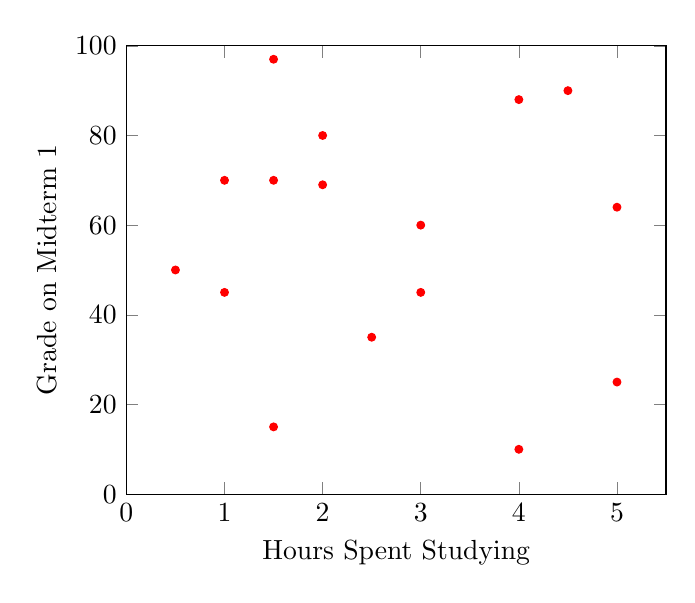
\begin{tikzpicture} 
\begin{axis}[
	xlabel = {Hours Spent Studying},
	ylabel = {Grade on Midterm $1$},
	xmin = {0},
	ymin = {0},
	ymax = {100}
	]
\addplot[only marks, red, mark = *, mark size = 1.4pt] coordinates{
	(1, 70) (2, 80) (1.5, 97) (0.5, 50) (1.5, 70) (4, 88) (3, 60) (4, 10) (5, 64) (5,25) (3, 45) (4.5, 90) (1, 45) (2, 69) (2.5, 35) (1.5, 15)};
%\addplot[samples = 50]{20*x + 2};
\end{axis} \end{tikzpicture} $$ 

\easysubproblem{Give an example of two variables that are not correlated nor associated by drawing a plot.}\spc{4}
$$ 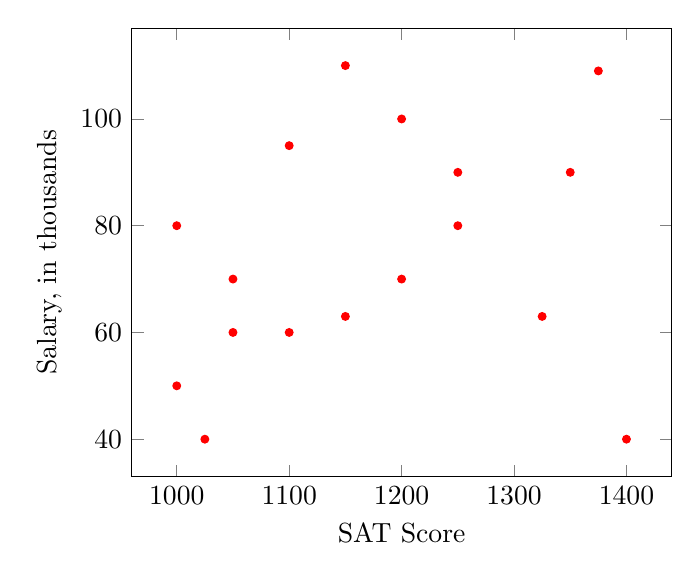
\begin{tikzpicture} 
\begin{axis}[
	xlabel = {SAT Score},
	ylabel = {Salary, in thousands},
	xticklabels = {800,1600},
	yticklabels = {20, 100},
	xticklabels = {800, 900, 1000, 1100, 1200, 1300, 1400},
	yticklabels = {0, 20, 40, 60, 80, 100, 120}
	]
\addplot[only marks, red, mark = *, mark size = 1.4pt] coordinates{
	(850, 20) (800, 30) (800, 60) (900, 50) (900, 40) (1000, 40) (1000, 75) (1100, 90) (1100, 43) (1200, 50) (1200, 80) (1300, 70) (1300, 60) (1450, 43) (1500, 70) (1600, 20) (1550, 89)};
\end{axis} \end{tikzpicture} $$ 
\easysubproblem{Can two variables be correlated but not associated? Explain.}\spc{4} \\ 
Two variables can be correlated but not associated due to sheer coincidence. For example, suppose as ice cream sales increased, the rate of drowning deaths increased sharply. Therefore ice cream consumption causes drowning. These two variables are positively correlated but have nothing to do with each other. It could be that ice cream sales are high during summer months as well as water activities. But drowning deaths are only caused by more exposure to water based activities, not ice cream. 


\end{enumerate} \newpage

\problem{These are questions about multivariate linear model fitting using the least squares algorithm.}

\begin{enumerate}

\hardsubproblem{Derive $\partialop{\c}{\c^\top A \c}$ where $\c \in \reals^n$ and $A \in \reals^{n \times n}$ but \textit{not} symmetric. Get as far as you can.}\spc{8}
First find $A\c$, $$ A\c= \begin{bmatrix} a_{11} & a_{12} & \dots & a_{1n} \\ a_{21} & a_{22} & \dots & a_{2n} \\ \vdots & \vdots & \ddots & \vdots \\ a_{n1} & a_{n2} & \dots & a_{nn} \end{bmatrix} \begin{bmatrix} c_1 \\ c_2 \\ \vdots \\ c_n \end{bmatrix} = \begin{bmatrix} a_{11}c_1 + a_{12}c_2 + \dots + a_{1n}c_n \\ a_{21}c_1 + a_{22}c_2 + \dots + a_{2n}c_n \\ \vdots \\ a_{n1}c_1 + a_{n2}c_2 + \dots + a_{nn}c_n \end{bmatrix} $$ 
Then 
$$ \begin{aligned} \c^\top A\c &= \begin{bmatrix} c_1 & c_2 & \dots & c_n \end{bmatrix} \begin{bmatrix} a_{11}c_1 + a_{12}c_2 + \dots + a_{1n}c_n \\ a_{21}c_1 + a_{22}c_2 + \dots + a_{2n}c_n \\ \vdots \\ a_{n1}c_1 + a_{n2}c_2 + \dots + a_{nn}c_n \end{bmatrix} \\ &= c_1(a_{11}c_1 + a_{12}c_2 + \dots + a_{1n}c_n) \\ &+ c_2(a_{21}c_1 + a_{22}c_2 + \dots + a_{2n}c_n) \\ &+ \dots + c_n(a_{n1}c_1 + a_{n2}c_2 + \dots + a_{nn}c_n) \end{aligned} $$ 
Note that $$ \partialop{c_1}{\c^\top A\c} = a_{11}c_1 + (a_{11}c_1 + a_{12}c_2 + \dots + a_{1n}c_n) + a_{21}c_2 + a_{31}c_3 + \dots + a_{n1}c_n $$ 
Let's do the next row to note the pattern 
$$ \partialop{c_2}{\c^\top A\c} = a_{12}c_1 + a_{22}c_2 + (a_{21}c_1 + a_{22}c_2 + \dots + a_{2n}c_n) + a_{32}c_3 + \dots + a_{n2}c_n$$ 
Since $A$ is not symmetric, we cannot clean this up and can only write it as a form of summations $$ \begin{aligned} \partialop{c_1}{\c^\top A\c} &= \sum a_{1i}c_i + \sum a_{i1}c_i = \sum (a_{1i} + a_{i1})c_1\\ \partialop{c_2}{\c^\top A\c} &= \sum a_{2i}c_i + \sum a_{i2}c_i = \sum (a_{2i} + a_{i2})c_2 \end{aligned} $$ 
Therefore $$ \partialop{\c}{\c^\top Ac} = \begin{bmatrix} \sum (a_{1i} + a_{i1})c_1 \\ \sum (a_{2i} + a_{i2})c_2 \\ \vdots \\ \sum (a_{ni} + a_{in})c_n \end{bmatrix} $$ 

\newpage
\easysubproblem{Given matrix $X \in \reals^{n \times (p+1)}$, full rank and first column consisting of the $\onevec_n$ vector, rederive the least squares solution $\b$ (the vector of coefficients in the linear model shipped in the prediction function $g$). No need to rederive the facts about vector derivatives.}\spc{10} \\
First let's find a closed form for SSE: $$ \begin{aligned} 
SSE &= \sum_{i=1}^n (y_i - \hat{y}_i)^2 \\ &= (\vec{y} - \vec{\hat{y}})^\top(\vec{y} - \vec{\hat{y}}) = (\vec{y}^\top - \vec{\hat{y}}^\top)(\vec{y} - \vec{\hat{y}}) \\ &= \vec{y}^\top\vec{y} - \vec{\hat{y}}^\top\vec{y} - \vec{y}^\top\vec{\hat{y}} + \vec{\hat{y}}^\top\vec{\hat{y}} \\ &= \vec{y}^\top\vec{y} - 2\vec{\hat{y}}^\top\vec{y} + \vec{\hat{y}}^\top\vec{\hat{y}} \\ &= \vec{y}^\top\vec{y} - 2(X\vec{w})^\top\vec{y} + (X\vec{w})^\top(X\vec{w}) \\ &= \vec{y}^\top\vec{y} - 2\vec{w}^\top X^\top\vec{y} + \vec{w}^\top X^\top X\vec{w} \end{aligned} $$ 
Integrate this with respect to $\vec{w}$ to attain $\b$: $$ \begin{aligned} \frac{\partial}{\partial \vec{w}} SSE &= \frac{\partial}{\partial \vec{w}} (\vec{y}^\top \vec{y} - 2\vec{w}^\top X^\top\vec{y} + \vec{w}^\top X^\top X\vec{w}) \\ &= \frac{\partial}{\partial \vec{w}} (\vec{y}^\top\vec{y}) - 2\frac{\partial}{\partial \vec{w}} (\vec{w}^\top X^\top\vec{y}) + \frac{\partial}{\partial \vec{w}} (\vec{w}^\top X^\top X\vec{w}) \\ &= \vec{0} - 2X^\top\vec{y} + 2X^\top X\vec{w} \stackrel{\text{set}}{=} 0 \\ X^\top\vec{y} &= X^\top X\vec{w} \\ \w = \b &= (X^\top X)^{-1}X^\top\vec{y} \end{aligned} $$ 

\intermediatesubproblem{Consider the case where $p = 1$. Show that the solution for $\b$ you just derived is the same solution that we proved for simple regression in Lecture 8. That is, the first element of $\b$ is the same as $b_0 = \ybar - r \frac{s_y}{s_x}\xbar$ and the second element of $\b$ is $b_1 = r \frac{s_y}{s_x}$.} \spc{10} \\
Let $X \in \reals^{n \times (1+1)} = \reals^{n \times 2}$. This looks like $\begin{bmatrix} 1_n & \vec{x} \end{bmatrix}$. Additionally, $\vec{y}$ is a column of $n$ values of $y$s. Take tthe above solution one piece at a time. First let's compute $X^\top X$. This is 
$$ X^\top X = \begin{bmatrix} 1 & 1 & \dots & 1 \\ x_1 & x_2 & \dots & x_n \end{bmatrix} \begin{bmatrix} 1 & x_1 \\ 1 & x_2 \\ \vdots & \vdots \\ 1 & x_n \end{bmatrix} 
= \begin{bmatrix} n & \sum x_i \\ \sum x_i & \sum x_i^2 \end{bmatrix} $$ 
The inverse of $X^\top X$ is $$ (X^\top X)^{-1} = \begin{bmatrix} n & \sum x_i \\ \sum x_i & \sum x_i^2 \end{bmatrix}^{-1} = \begin{bmatrix} \frac{\sum x_i^2}{n\sum (x_i - \bar{x})^2} & -\frac{\sum x_i}{n\sum (x_i - \bar{x})^2} \\ -\frac{\sum x_i}{n\sum (x_i - \bar{x})^2} & \frac{n}{n\sum (x_i - \bar{x})^2} \end{bmatrix} = \begin{bmatrix} \frac{1}{n} + \frac{\bar{x}^2}{\sum (x_i - \bar{x})^2} & -\frac{\bar{x}}{\sum (x_i - \bar{x})^2} \\ -\frac{\bar{x}}{\sum (x_i - \bar{x})^2} & \frac{1}{\sum (x_i - \bar{x})^2} \end{bmatrix} $$ 
Before finding $\b$, first find $X^\top \vec{y}$, which is 
$$ X^\top \vec{y} = \begin{bmatrix} 1 & 1 & \dots & 1 \\ x_1 & x_2 & \dots & x_n \end{bmatrix} \begin{bmatrix} y_1 \\ y_2 \\ \vdots \\ y_n \end{bmatrix} = \begin{bmatrix} \sum y_i \\ \sum x_iy_i \end{bmatrix} $$ 
Thus $$ \begin{aligned} \b &= (X^\top X)^{-1} (X^\top \vec{y}) \\ &= \begin{bmatrix} \frac{1}{n} + \frac{\bar{x}^2}{\sum (x_i - \bar{x})^2} & -\frac{\bar{x}}{\sum (x_i - \bar{x})^2} \\ -\frac{\bar{x}}{\sum (x_i - \bar{x})^2} & \frac{1}{\sum (x_i - \bar{x})^2} \end{bmatrix} \begin{bmatrix} \sum y_i \\ \sum x_iy_i \end{bmatrix} \\ &= \begin{bmatrix} \frac{\sum y_i}{n} + \frac{\sum y_i \bar{x}^2}{\sum (x_i - \bar{x})^2} - \frac{ \sum x_iy_i\bar{x}}{\sum (x_i - \bar{x})^2} \\ -\frac{\sum y_i \bar{x}}{\sum (x_i - \bar{x})^2} + \frac{x_iy_i}{\sum (x_i - \bar{x})^2} \end{bmatrix} \\ &= \begin{bmatrix} \bar{y} - b_1\bar{x} \\ \frac{\sum y_i(x_i - \bar{x})}{\sum (x_i - \bar{x})^2} \end{bmatrix} \\ &= \begin{bmatrix} b_0 \\ b_1 \end{bmatrix} \end{aligned} $$ 


\easysubproblem{If $X$ is rank deficient, how can you solve for $\b$? Explain in English.} \spc{2} \\
If $X$ is rank deficient, then there is duplicated data where one or more columns are a linear combination of the other columns in $X$. To solve for $\b$, remove the duplicated columns so that all the columns are linearly independent. 

\hardsubproblem{Prove $\rank{X} =\rank{X^\top X}$.}\spc{6} \\
Let $X$ has rank and let $x \in N(X)$ where $N(X)$ is the null space of $X$. The null space of $X$ is such that $xX = 0$. If $\rank{X} = \rank{X^\top X}$, then $x$ is in the null space of $X^\top X$, or $x \in N(X^\top X)$. Hence $N(X) \subseteq N(X^\top X)$. Now suppose $x \in N(X^\top X)$, the null space of $X^\top X$. Then $$ \begin{aligned} X^\top Xx &= 0 \\ x^\top X^\top Xx &= 0 \\ (Xx)^\top (Xx) &= 0 \\ Xx &= 0 \end{aligned} $$ Here we find that $x$ is in the null space of $X$, or $x \in N(X)$. Therefore $N(X^\top X) \subseteq N(X)$. Furthermore, $$ \begin{aligned} N(X^\top X) &= N(X) \\ \dim[N(X^\top X)] &= \dim[N(X)] \\ \rank{X^\top X} &= \rank{X} \end{aligned} $$ 

\newpage
\hardsubproblem{Given matrix $X \in \reals^{n \times (p+1)}$, full rank and first column consisting of the $\onevec_n$ vector, now consider cost multiples (\qu{weights}) $c_1, c_2, \ldots, c_n$ for each mistake $e_i$. As an example, previously the mistake for the 17th observation was $e_{17} := y_{17} - \hat{y}_{17}$ but now it would be $e_{17} := c_{17} (y_{17} - \hat{y}_{17})$.  Derive the weighted least squares solution $\b$. No need to rederive the facts about vector derivatives. Hints: (1) show that SSE is a quadratic form with the matrix $C$ in the middle (2) Split this matrix up into two pieces i.e. $C = C^{\half} C^{\half}$, distribute and then foil (3) note that a scalar value equals its own transpose and (4) use the vector derivative formulas.}\spc{20} \\
First find a closed from for SSE: $$ \begin{aligned} 
SSE &= \sum c_i(y_i - \hat{y}_i)^2 \\ &= (\vec{y} - \vec{\hat{y}})^\top C(\vec{y} - \vec{\hat{y}}) \\ &= (\vec{y}^\top - \vec{\hat{y}}^\top)C(\vec{y} - \vec{\hat{y}}) \\ &= (\vec{y}^\top - \vec{\hat{y}}^\top)C^{\half}C^{\half}(\vec{y} - \vec{\hat{y}}) \\ &= (\vec{y}^\top C^{\half} - \vec{\hat{y}}^\top C^{\half})(C^{\half}\vec{y} - C^{\half}\vec{\hat{y}}) \\ &= \vec{y}^\top C^{\half}C^{\half}\vec{y} - \vec{\hat{y}}^\top C^{\half} C^{\half}\vec{y} - \vec{\hat{y}}^\top C^{\half} C^{\half} \vec{y} + \vec{\hat{y}}^\top C^{\half} C^{\half} \vec{\hat{y}} \\ &= \vec{y}^\top C\vec{y} - 2\vec{\hat{y}}^\top C\vec{y} + \vec{\hat{y}}^\top C \vec{\hat{y}} \\ &= \vec{y}^\top C\vec{y} - 2(X\vec{w})^\top C\vec{y} + (X\vec{w})^\top C (X\vec{w}) \\ &= \vec{y}^\top C\vec{y} - 2\vec{w}^\top X^\top C\vec{y} + \vec{w}^\top X^\top C X\vec{w} \end{aligned} $$ 
Integrate this with respect to $\vec{w}$ to attain $\b$: 
$$ \begin{aligned} \frac{\partial}{\partial \vec{w}} SSE &= \frac{\partial}{\partial \vec{w}} (\vec{y}^\top C\vec{y} - 2\vec{w}^\top X^\top C\vec{y} + \vec{w}^\top X^\top C X\vec{w}) \\ &= \frac{\partial}{\partial \vec{w}} (\vec{y}^\top C\vec{y}) - 2 \frac{\partial}{\partial \vec{w}} (\vec{w}^\top X^\top C\vec{y}) + \frac{\partial}{\partial \vec{w}} (\vec{w}^\top X^\top C X\vec{w}) \\ &= \vec{0} - 2X^\top C\vec{y} + 2X^\top CX\vec{w} \stackrel{\text{set}}{=} 0 \\ X^\top CX\vec{w} &= X^\top C\vec{y} \\ \b &= \vec{w} = (X^\top CX)^{-1}X^\top C\vec{y}
\end{aligned} $$ 

\newpage
\hardsubproblem{If $p=1$, prove $r^2 = R^2$ i.e. the linear correlation is the same as proportion of sample variance explained in a least squares linear model.}\spc{6} \\
Suppose $y = b_0 + b_1x$. Then $r^2 = \frac{\sum (\hat{y}_i - \bar{y})^2}{\sum (y_i - \bar{y})^2}$. Note that $b_1 = \frac{\sum (x_i - \bar{x})(y_i - \bar{y})}{\sum (x_i - \bar{x})^2}$. and $b_0 = \bar{y} - b_1\bar{x}$. Then $$ \begin{aligned} \sum (\hat{y}_i - \bar{y})^2 &= \sum (b_0 + b_1x_i - \bar{y})^2 \\ &= \sum (\hat{y} - b_1\bar{x} + b_1x_i - \bar{y})^2 \\ &= b_1^2 \sum (x_i - \bar{x})^2 \\ &= \frac{\sum (x_ i -\bar{x})(y_i - \bar{y})^2}{\sum (x_i - \bar{x})^2} \sum (x_i - \bar{x})^2 \\ &= \frac{[\sum (x_i - \bar{x})(y_i - \bar{y})]^2}{\sum (x_i - \bar{x})^2} \end{aligned} $$ 
Therefore $$ \begin{aligned} r^2 &= \frac{\sum (\hat{y}_i - \bar{y})^2}{\sum (y_i - \bar{y})^2} \\ &= \frac{[\sum (x_i - \bar{x})(y_i - \bar{y})]^2}{\sum (x_i - \bar{x})^2 \sum (y_i - \bar{y})^2} \\ &= \left( \frac{\sum (x_i - \bar{x})(y_i - \bar{y})}{\sqrt{\sum (x_i - \bar{x})^2 \sum (y_i - \bar{y})^2}}\right)^2 \\ &= R^2 \end{aligned} $$ 

\intermediatesubproblem{Prove that the point $\langle 1,\xbar_1, \xbar_2, \ldots, \xbar_p, \bar{y} \rangle$ is a point on the least squares linear solution.}\spc{13} \\
$$\vec{y} = \begin{bmatrix} y_1 \\ y_2 \\ \vdots \\ y_p \end{bmatrix} = \begin{bmatrix} b_0 + b_1x_{11} + \dots + b_px_{1p} \\ b_0 + b_1x_{21} + \dots + b_px_{2p} \\ \vdots \\ b_0 + b_1x_{p1} + \dots + b_px_{pp} \end{bmatrix} = X\b $$ 
Then $$ \begin{aligned} \sum_{i=1}^p y_i &= \sum_{i=1}^p (b_0 + b_1x_{i1} + \dots + b_px_{ip}) \\ \frac{ \sum y_i }{n} &= \frac{\sum (b_0 + b_1x_{i1} + \dots + b_px_{ip})}{n} \\
\frac{\sum y_i}{n} &= \frac{\sum b_0}{n} + \frac{\sum b_1x_{i1}}{n} + \dots + \frac{\sum b_px_{ip}}{n} \\ \frac{\sum y_i}{n} &= \frac{nb_0}{n} + \frac{nb_1\xbar_1}{n} + \dots + \frac{nb_p\xbar_p}{n} \\ \ybar &= b_0 + b_1\xbar_1 + \dots + b_p\xbar_p \end{aligned} $$ 

\end{enumerate}

\problem{These are questions related to the concept of orthogonal projection, QR decomposition and its relationship with least squares linear modeling.}

\begin{enumerate}

\easysubproblem{Consider least squares linear regression using a design matrix $X$ with rank $p + 1$. What are the degrees of freedom in the resulting model? What does this mean?}\spc{3} \\
The degrees of freedom in the resulting model is $p+1$. It means that there are $p+1$ independent variables to pick to describe $\y$. 

\intermediatesubproblem{If you are orthogonally projecting the vector $\y$ onto the column space of $X$ which is of rank $p + 1$, derive the formula for $\proj{\colsp{X}}{\y}$. Is this the same as the least squares solution?}\spc{6} \\
Project $\y$ onto the column space of $X$. 
$$ \begin{aligned} X\b &= \y \\ \vec{x}_1^\top (X\b - \y) &= 0 \\ \vec{x}_2^\top (X\b - \y) &= 0 \\ \vec{x}_n^\top (X\b - \y) &= 0 \end{aligned} $$ 
This means $$ \begin{aligned} X^\top (X\b - \y) &= 0 \\ X^\top X\b &= X^\top \y \\ \b &= (X^\top X)^{-1}X^\top \y \\ X\b &= X(X^\top X)^{-1}X^T\y \\ \proj{\colsp{X}}{\y} &= X(X^\top X)^{-1} X^\top \y \end{aligned} $$ 
This result is the same as the least squares solution.

\hardsubproblem{We saw that the perceptron is an \textit{iterative algorithm}. This means that it goes through multiple iterations in order to converge to a closer and closer $\w$. Why not do the same with linear least squares regression? Consider the following. Regress $\y$ using $\X$ to get $\yhat$. This generates residuals $\e$ (the leftover piece of $\y$ that wasn't explained by the regression's fit, $\yhat$). Now try again! Regress $\e$ using $\X$ and then get new residuals $\e_{new}$. Would $\e_{new}$ be closer to $\zerovec_n$ than the first $\e$? That is, wouldn't this yield a better model on iteration \#2? Yes/no and explain.}\spc{10} \\
This would not yield a better model on iteration \#2. After $\y$ is regressed using $\X$ to get $\yhat$, it is projected onto the space orthogonal to $X$, or the residual space. Then regressing $\e$ using $\X$ will result in the same projection with no new residuals because it is already in the space orthogonal to $\X$. \qu{$\e_{new}$} would not be closer to $\zerovec_n$ but will be the same as $\e$. 

\newpage
\intermediatesubproblem{Prove that $Q^\top = Q^{-1}$ where $Q$ is an orthonormal matrix such that $\colsp{Q} = \colsp{X}$ and $Q$ and $X$ are both matrices $\in \reals^{n \times (p+1)}$. Hint: this is purely a linear algebra exercise.}\spc{10} \\
If $Q$ is an orthonormal matrix, then for any two vectors $q_i,q_j \in Q$, $q_i^\top q_j = \begin{cases} 0 &\text{ if } i \neq j \\ 1 &\text{ if } i = i \end{cases}$. This means that each vector is perpendicular to each other. Henceforth $$Q^\top Q = \begin{bmatrix} 1 & 0 & \dots & 0 \\ 0 & 1 & \dots & 0 \\ \vdots & \vdots & \ddots & \vdots \\ 0 & 0 & \dots & 1 \end{bmatrix} = I_n $$ 
If so, then $$ \begin{aligned} Q^\top Q &= I_n \\ (Q^\top Q)Q^{-1} &= I_n Q^{-1} \\ Q^\top &= Q^{-1} \end{aligned} $$ 


\intermediatesubproblem{Prove that the least squares projection $H = \XXtXinvXt$ is the same as $QQ^\top$.}\spc{10} \\
Note that $H = \XXtXinvXt$. Let $X=Q$.  $$\vec{\hat{y}} = H\vec{y} = X(X^\top X)^{-1}X^\top \vec{y} = Q(Q^\top Q)^{-1}Q^\top \vec{y}$$
From the last problem, we see that $Q^\top Q = I_n$. Then 
$$\vec{\hat{y}} = Q(Q^\top Q)^{-1} Q^\top \vec{y} = Q(I_n)^{-1}Q^\top\vec{y} = QQ^\top \vec{y}$$
Hence $X(X^\top X)^{-1}X^\top = QQ^\top$. 




\intermediatesubproblem{Prove that an orthogonal projection onto the $\colsp{Q}$ is the same as the sum of the projections onto each column of $Q$.}\spc{10} \\
Divide the projection component wise
 $$ \begin{aligned} \proj{\colsp{X}}{\y} &= \proj{\vec{x}_1}{\y} + \proj{\vec{x}_2}{\y} + \dots + \proj{\vec{x}_n}{\y} \\ &= \frac{\vec{x}_1\vec{x}_1^\top}{\norm{\vec{x}_1}^2}\y + \frac{\vec{x}_2\vec{x}_2^\top}{\norm{\vec{x}_2}^2}\y + \dots + \frac{\vec{x}_n\vec{x}_n^\top}{\norm{\vec{x}_n}^2}\y \\ &= \left( \frac{\vec{x}_1\vec{x}_1^\top}{\norm{\vec{x}_1}^2} + \frac{\vec{x}_2\vec{x}_2^\top}{\norm{\vec{x}_2}^2} + \dots + \frac{\vec{x}_n\vec{x}_n^\top}{\norm{\vec{x}_n}^2}\right)\y \end{aligned} $$ 
Note that $X$ is orthonormal and so 
$$ \begin{aligned} \proj{\colsp{X}}{\y} &= (\vec{x}_1\vec{x}_1^\top + \vec{x}_2\vec{x}_2^\top + \dots + \vec{x}_n\vec{x}_n^\top)\y \\ &= \Biggl(\begin{bmatrix} x_{11}^2 & x_{11}x_{12} & \dots & x_{11}x_{1n} \\ x_{12}x_{11} & x_{12}^2 & \dots & x_{12}x_{1n} \\ \vdots & \vdots & \ddots & \vdots \\ x_{1n}x_{11} & x_{1n}x_{12} & \dots & x_{1n}^2 \end{bmatrix} + \begin{bmatrix} x_{21}^2 & x_{21}x_{22} & \dots & x_{21}x_{2n} \\ x_{22}x_{21} & x_{22}^2 & \dots & x_{22}x_{2n} \\ \vdots & \vdots & \ddots & \vdots \\ x_{2n}x_{21} & x_{2n}x_{22} & \dots & x_{2n}^2 \end{bmatrix} \\ &+ \dots + \begin{bmatrix} x_{n1}^2 & x_{n1}x_{n2} & \dots & x_{n1}x_{nn} \\ x_{n2}x_{n1} & x_{n2}^2 & \dots & x_{n2}x_{nn} \\ \vdots & \vdots & \ddots & \vdots \\ x_{nn}x_{n1} & x_{nn}x_{n2} & \dots & x_{nn}^2 \end{bmatrix}\Biggr)\y \\ &= \left( \begin{bmatrix} \uparrow & \uparrow & \dots & \uparrow \\ \vec{x}_1 & \vec{x}_2 & \dots & \vec{x}_n \\ \downarrow & \downarrow & \dots & \downarrow \end{bmatrix} \begin{bmatrix} \leftarrow & \vec{x}_1^\top & \rightarrow \\ \leftarrow & \vec{x}_2^\top & \rightarrow \\ \vdots & \vdots & \vdots \\ \leftarrow & \vec{x}_n^\top & \rightarrow \end{bmatrix}\right)\y \\ &= QQ^\top\y \\ &= \proj{\colsp{X}}{\y} \end{aligned} $$ 

\hardsubproblem{Trouble in paradise. Prove that the SSE of a multivariate linear least squares model always decreases (equivalently, $R^2$ always increases) upon the addition of a new independent predictor. Keep in mind this holds true even if this new predictor has no information about the true causal inputs to the phenomenon $y$.}\spc{12} \\
Recall that $$SSR = \sum \hat{y}_i - n\bar{y}^2 = \sum_{j=1}^p \norm{\proj{\vec{x}_j}{\vec{y}}}^2 - n\bar{y}^2 $$ If a new predictor $\vec{x}_{new}$ is added to $X$, then 
$$SSR_{new} = \left(\sum_{j=1}^p \norm{\proj{\vec{x}_j}{\vec{y}}}\right) + \underbrace{\norm{\proj{\vec{x}_{new}}{\vec{y}}}^2}_{> 0} - n\bar{y}^2 $$ 
Since the new term added is positive, this means that $SSR_{new} > SSR$ and since $SST = SSR + SSE$ is constant, $$SSE_{new} < SSE$$ Therefore the SSE decreased. Furthermore, $$ \begin{aligned} 
SSR_{new} &> SSR \\ \frac{SSR_{new}}{SST} &> \frac{SSR}{SST} \\ R^2_{new} &> R^2 \end{aligned} $$ Thus $R^2$ always increases upon the addition of a new independent predictor. 

\intermediatesubproblem{Why is this a bad thing? Explain in English.}\spc{3} \\
This is a bad thing because if we keep adding new useless inputs, we will be able to attain $R^2 = 100\%$ where $100\%$ of the variance will be explained. But all this variance will be explained by the help of random data points that has nothing to contribute to the phenomenon. The model will be overfit due to unhelpful data. 


\extracreditsubproblem{Prove that $\rank{H} =\tr{H}$.}\spc{-0.5} \\
Preliminary step: Show $\tr{AB} = \tr{BA}$. 
$$ \begin{aligned} \tr{AB} &= \sum_{i=1}^n (AB)_{ii} \\ &= \sum_{i=1}^n\sum_{j=1}^n A_{ij}B_{ji} \\ &= \sum_{j=1}^n \sum_{i=1}^n B_{ji}A_{ij} \\ &= \sum_{j=1}^n (BA)_{jj} \\ &= \tr{BA} \end{aligned} $$ 
Therefore, if $\rank{H} = n+1$, prove that $\tr{H} = n+1$. 
$$ \begin{aligned} \tr{H} &= \tr{X(X^\top X)^{-1} X^\top} \\ &= \tr{(X^\top X)^{-1}X^\top X} \\ &= \tr{Z^{-1}Z} \\ &= \tr{I} \\ &= n+1 \end{aligned} $$ 

\end{enumerate}


\end{document}